
\chapter{General introduction}
\label{introduction}

\begin{abstract}
In this chapter, we introduce the concept of lyotropic liquid crystals from both a practical and statistical mechanical perspective. Additionally, we discuss some topics related to Monte Carlo simulations in the semi-grand-canonical ensemble. We also outline the goal of this thesis in relation to recent experimental research on the self-organization of anisotropic colloidal nanoparticles in complex environments.

\end{abstract}


\section{Phenomenological background}

{\em Soft matter} is a term used to describe materials that are distinct from gases and solids, usually excluding simple fluids. A wide range of systems, including soap bubbles, gels, elastomers, liquid crystals, or biological fluids, can be categorized as soft matter. Defining the boundaries of such a vast domain can be challenging due to the diverse topics and segregated nature of researchers, which come from a number of distinct disciplines. Nevertheless, a clear community with a common language exists, and major research topics can be identified that encompass most current studies in this field \cite{borsali2018soft}.

Soft matter systems exhibit, in most cases, structural length scales ranging from a nanometer up to a micrometer, and thus are placed within the domain of ‘nanotechnology’. Colloidal systems are well known examples in which this feature is essential to define the range where a very specific type of behavior occurs. Colloids are supramolecular submicron sized substances dispersed in a medium that can be a liquid or a gas. They are much bigger than normal molecules, and hence the medium in a colloidal suspension can often be regarded as ‘background’ with respect to the colloidal size range: this medium may be approximated as a continuum. At the same time, colloids are small enough to present considerable thermal motion in comparison to sedimentation (which is caused by gravitational forces that would become more important for higher-sized particles). Colloids were first discovered by Perrin, who detected Brownian motion as visible manifestation of thermal motion in dispersions of resin colloids in water \cite{perrin1913atomes}.

When colloidal particles have anisotropic shapes, they can be found in liquid crystalline phases. Liquid crystals are substances that have the appearance of a liquid but possess certain levels of molecular arrangement similar to crystals. Liquid crystals were first discovered in 1888 by Friedrich Reinitzer, who noticed that a cholesterol-based substance had two melting points at different temperatures, each of them giving way to a liquid-like phase with different optical properties \cite{reinitzer1888beitrage}. At the early time of Reinitzer only three phases were known (gas, liquid and solid). Over the years, a big number of substances have been discovered to exhibit many states of matter, including liquid crystal phases that are now widely used in technological advancements such as liquid crystal screens and thermometers \cite{Li_2012}.

The key difference between a liquid crystal and the commonly observed gas, liquid and solid states is that properties in the first one are anisotropic and vary with direction, even though the substance itself remains fluid. These unique properties emerge due to the elongated shape of its building blocks, which promote collective alignment along a certain direction. In other words, liquid crystalline phases are additional states of matter which are intermediate between the dilute gas and the crystalline solid, and whose existence is related to the additional {\em orientational} degrees of freedom anisometric particles have compared to spherical ones.

\begin{figure}
\begin{center}
\includegraphics[width= \columnwidth]{figures/chapter-1/phases}
\caption[Examples of basic liquid crystals formed by rod-like molecules or nanoparticles.]{ \label{introfig1} (a)-(d) Examples of basic liquid crystals formed by rod-like molecules or nanoparticles. (e) Most molecular chiral features in elongated nano-particles  could be described on a coarse-grained level using a rod with an effective chiral electrostatic ``patchiness"  in terms of a molecular pitch length and handedness (left or right); (f) these particles generate a particular type of nematic phase: the chiral nematic. The implications of molecular chirality on the helical mesostructure (in particular, the mesoscopic pitch) of chiral nematic phases remains a challenging issue.}
\end{center}
\end{figure}

Among the numerous liquid crystalline phases, different degrees of order can be found, evidenced for instance by diffraction of X-rays and light. Measurements of this kind provide a frame to classify these systems by its similarity to either the gas or the solid phase. Let us consider, among others, the following liquid crystalline phases, depicted in \fig{introfig1}:

The {\em isotropic} (I) fluid phase is very similar to the gas and liquid phases for spherical particles and is characterized by a complete absence of positional and orientational order. At the inmediately next stage, we find the {\em nematic} (N) phase, in which particles are homogeneously distributed without positional order as in a liquid phase, but are ordered in their orientation following an average direction: the {\em nematic director} $\bn$. As it will be repeatedly discussed throughout this thesis, in nature one can find particles that, in addition to being anisotropic, present chiral features. This can be due to the arrangement of atoms in a molecular compound, to a (helicoidal) particle shape in some colloidal systems or to a chiral distribution of charges at the surface of the particles, observed for instance in {\em fd} filamentous bacteriophages viral rods \cite{Gibaud_2017}. When chiral particles are in nematic phase, they arrange themselves into a strongly twisted structure. This special case of a nematic phase is often called {\em cholesteric}.

The {\em smectic} (Sm) phase is closer to the solid phase. In smectic liquid crystals, particles are ordered in layers and cannot move freely between them. The smectic phase is, in turn, divided into several sub-phases with slightly different properties. Examples are the smectic A phase (SmA), where particles can move freely inside the layers as in a two-dimensional liquid; or the smectic B phase (SmB), where there is long-ranged positional order: at higher concentrations or lower temperatures, molecules tend to arrange themselves into something more similar to a crystalline lattice.

One sub-classification of liquid crystal materials is based on the mechanism by which they transition from one state to another. {\em Thermotropic} systems, mainly formed by low molecular weight constituents --and also some polymers--, undergo phase transitions due to changes in temperature, since the thermodynamic properties of these species depend on the attractive forces between the molecules. In this thesis, we focus mostly on  {\em lyotropic} liquid crystals, which form upon increasing the concentration of solute particles. This is the case of systems formed by high-molecular weight synthetic and biological nano-particles \cite{sonin1998inorganic,dogic-fraden_fil}, polymers such as DNA \cite{livolantDNAoverview} or surfactants in a solvent \cite{fontell1981}. The first case is the one studied in this thesis, where the fact that shape is not subject to fluctuations due to changes in the solvent composition is an advantageous simplification with respect to its amphiphilic and polymeric counterparts.

First experimental reports of nano-particle based lyotropic liquid crystals go back when liquid crystalline behaviour was described for tobacco and tomato mosaic virus (TMV) \cite{Bawden,Bernal} and vanadium pentoxide (V$_{2}$O$_{5}$) \cite{Zocher} in the early 20th century. In addition to these rod-like particle systems, colloidal plate-like charged particles and clay particles were discovered to report liquid crystalline behaviour \cite{Langmuir}. At present, there are many other examples of lyotropic liquid crystals to be found in a wide variety of dispersions of (mainly rod-like) colloidal particles and solutions of stiff polymers (see e.g. \cite{Dierking2020} for an overview).

This research work focuses on both theoretical and numerical approaches for the exploration of phase behavior in anisotropic colloidal compounds, with a particular interest in the {\em entropic} isotropic-nematic phase transition. This transition is well described by Onsager's theory, proposed in 1949, which assumes a similarity between a gas and a particle solution \cite{onsager1949}; and will be used repeatedly throughout this manuscript (more specifically in Chapters \ref{disc_polymer} and \ref{hybridLC2}) along with other theoretical and numerical tools to study the liquid-crystalline self-organization of colloidal rods or platelets in complex environments. Through our research, we hope to gain a better understanding of the behavior of this kind of systems and contribute to the broader field of liquid crystal research.

\subsection{Entropic phase transitions}
\label{entropy_order}

The thermodynamic equilibrium state of a system tends to minimize its Helmholtz free energy:

\beq
F=U-TS
\label{genhelmholtz}
\eeq
where $U = \sum_{i \neq j} u_{ij}$ is the internal energy of the system defined as a pairwise addition of interparticle potentials $u_{ij}$ between particles $i$ and $j$, $T$ is the temperature and $S$ is the entropy of the system. Clearly, a system at constant temperature can lower its free energy in two ways: either by increasing the entropy or by decreasing the internal energy. Entropy is defined, for an isolated system of $N$ particles in a volume $V$ at an energy $U$, as follows:

\beq
S = k_B\log(\mbox{\# {\small accessible states}})
\eeq
and depends on the total number of states that are accessible to the system under these conditions. Usually, $S$ is interpreted as a measure for the ‘disorder’ in that system. The natural consequence of this interpretation would be that ordering phase transitions can only take place if the loss in entropy is compensated by the decrease in internal energy. These kind of phase transitions are known as {\em energetic} phase transitions and describe the reality, for example, of the spontaneous phase transition from the regular fluid to the solid crystalline state. In this case, the transition takes place if the freezing lowers the internal energy of the system sufficiently to offset the decrease in the number of accessible configurations and thus the loss in entropy.

However, we can have many ‘ordering’ transitions that are {\em entropic}. Taking \eq{genhelmholtz} one may consider systems in which the internal energy is a function of temperature alone, $S$ being the only quantity affected by any change in the system at constant temperature. If this is the case, it will be possible to find phase transformations determined exclusively by a change in the entropy. Usually, atomic systems do not fulfill this condition because of the existence of attractive or repulsive interactions $u_{ij}$ whose strength depends on the relative inter-particle distance, an thus, the number density of particles $\rho$ when considering the thermodynamic limit. Temperature is then key to determine the accessibility of an ordered state, following the Boltzmann probability of finding a particle configuration of energy U, $\exp( -U/k_{B}T)$. Nevertheless, if we limit our attention to hard-core potentials:

\beq
u_{ij}(r)=
\begin{cases}
\infty & r<D \textrm{ (if cores overlap)}\\
0 & r>D \textrm{ (if cores do not overlap)}
\end{cases}
\eeq
where $D$ is the diameter of the hard-core shell (which becomes an orientation-dependent quantity for anisotropic particles) and $r$ is the distance between centres of mass, then all the allowed (non-overlapping) configurations at constant temperature will possess the same level of internal energy $U=0$. Interestingly, $T$ then becomes completely irrelevant and any variation in the Helmholtz free energy will be attributed to changes in entropy, that will be maximized at equilibrium. Ordering phase transitions may occur in systems of this kind, e.g. in systems formed by rod-like particles, considering that entropy in these systems can be partitioned into two different components:

\beq
S = S_{trans} + S_{rot}
\eeq
where $S_{trans}$ is the translational entropy, related to accessible arrangements due to translational degrees of freedom and $S_{rot}$ is associated with the ways in which the particles can orient or rotate. The notion that spontaneous ordering of particles corresponds to an increase of the total entropy can be understood under this frame as a competition between these two quantities. When some kind of order emerges, particles lose entropy because the density --in terms of orientations-- is no longer uniform. However, this loss is more than offset by the simultaneous gain of translational entropy, i.e.  the available space per particle increases as the particles align. This argument can be extended to higher density phase transformations where positional order is achieved and the available volume each particle is allowed to explore increases if particles are arranged in a more ordered state instead of keeping a homogeneous positional distribution.

The isotropic-nematic phase transition invoked above occurs through a first order transition, as it was probed theoretically by Onsager. He recognized that the transition from an isotropic to a nematic state in solutions containing sufficiently anisometric particles can be described successfully  within a virial expansion of the free energy truncated after the second virial term, an approach which could not be used to explain the gas-liquid transition for spherical particles. About a decade after Onsager's work, Alder Wainwright and others \cite{ALDER57,WOOD57} first showed by means of computer simulations that a similar disorder-order transition, albeit of the positional degrees of freedom, occurs in a fluid of hard spheres, where there is a critical packing fraction at which particles will be able to better explore the translational phase space by adopting an (fcc) lattice rather than a disordered arrangement. Much later, computer simulations by Frenkel {\em et al.}  revealed the stability of smectic and columnar liquid crystals which appear upon densifying systems of respectively hard rods \cite{Frenkel88} and hard platelets \cite{FrenkelLiqcryst,Veerman},  without  attractive interactions between the particles. All of them consist of transitions driven entirely by {\em entropic} interactions.




\subsection{Mixtures and the depletion effect}

So far we have implicitly assumed that all particles which build up a gas, liquid (crystal) or solid phase are identical. Many systems in nature are however {\em mixtures} containing a number of different types of particles or molecules. It is not surprising that the phase behaviour of mixtures is richer than that of pure systems--if only for the additional {\em entropy of mixing}-- and that mixing different species may lead to  phenomena not encountered in one-component systems. An example of a purely entropically-driven self-assembly phenomenon is the ordered arrangement that arises in colloidal mixtures of large particles and smaller particles called depletants, a process known as the depletion effect.

\begin{SCfigure}
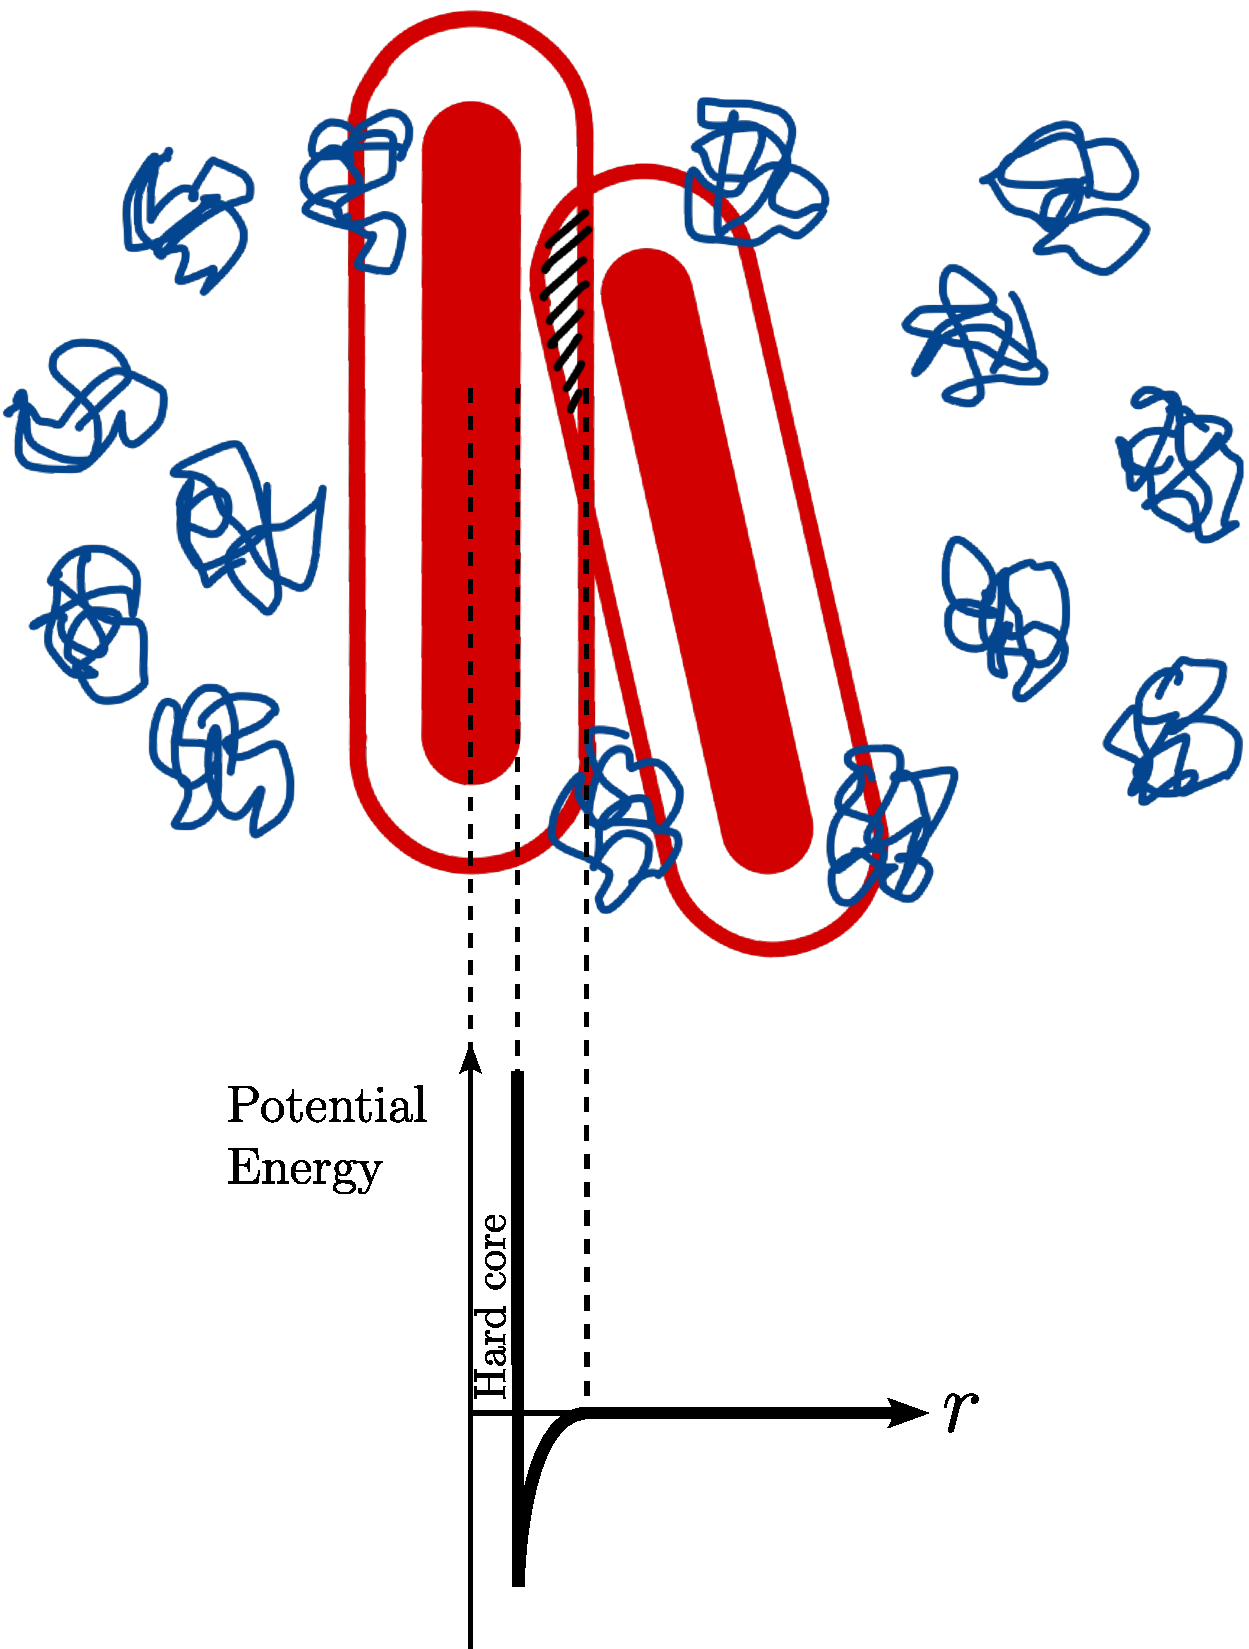
\includegraphics[width= 0.4 \columnwidth]{figures/chapter-1/depletion}
\caption[The presence of non-adsorbing polymers or other depletions agents (whose size is usually smaller than the colloidal nanoparticles)]{ \label{introfig2} The presence of non-adsorbing polymers or other depletions agents (whose size is usually smaller than the colloidal nanoparticles) produces an effective attractive potential between the rods according to the depletion scenario --which depends on the rods relative orientation and distance--. If the rods are at close proximity, the polymers are depleted away from the inner space between the rods in dictated by the overlap of the depletion zones (hatched area). This creates an osmotic imbalance around the cylindrical surfaces pushing the rods together.  }
\end{SCfigure}

This effect takes place typlically when colloidal particles are mixed with non-adsorbing polymers. \fig{introfig2} highlights the ordering transition in this situation by illustrating the effective attractive interaction between large colloidal rods when polymers are added to the system. Negative adsorption results in a region near the colloidal surface, named {\em depletion layer}, where polymers are less likely to access due to a loss of configurational entropy of the polymer chain. When such regions overlap, there is an increase in the volume available to polymers to explore, thus increasing their entropy and lowering their Helmholtz free energy. Effectively, the addition of depletants to the system generates repulsion between particles of distinct type and, in consequence, attraction between similarly-shaped colloidal particles.

These polymers are often modeled as penetrable hard spheres \cite{GARCIA201816}, known as Asakura-Oosawa spheres, in honor of the first theoreticians who proposed a model to describe the depletion effect \cite{ASAKURA54,ASAKURA58,Vrijdepletie}. By replacing the polymers with spheres of the same radius of gyration, we can obtain the same results in an effective manner. Penetrable hard objects do not interact with each other, i.e. no overlap restrictions are imposed between them, allowing for an ideal gas statistical mechanical treatment; and at the same time they are not allowed to overlap with colloidal particles, causing the emergence of the depletion effect. To sum up, the main approximations assumed by Asakura and Oosawa are: 1) whereas polymer chains in reality are unlikely found inside the depletion layers, in this model they are strictly prohibited; and 2) polymer chains are assumed to be completely transparent to each other, which is a fair approximation in the low depletant concentration regime.

In this work, depletion-driven demixing caused by strong shape assymetry in colloidal mixtures emerges in a natural way in Chapter \ref{disc_polymer} for a system featuring discs and polymerizing rods. In addition to it, the consequences of using penetrable hard spheres as a driving agent to stabilize liquid crystalline droplets will be deeply explored in Chapter \ref{twistedrods}.

\section{Scope of this thesis}

The central aim of this thesis is to theoretically investigate the liquid crystal (LC) self-organization of colloidal particles with different shapes in various contexts. Many of the studies to be described in the remainder of this thesis have been inspired by recent experimental works in systems of colloids with well-controlled shapes and interactions. In particular, we mention the experimental work of \cite{Grelet2014} on phase behavior and functionalization of complex fluids of filamentous bacteriophages (fd and M13) which display many interesting phenomena left open for theoretical interpretation; as well as recent experimental findings \cite{senyuk2021nematoelasticity,mundoor2021} on colloidal dispersion of highly anisotropic particles immersed in molecular LC hosts. One of our primary goals in this work is to account for these experimental observations by constructing simple, yet realistic,  models for the colloidal systems under consideration and by scrutinizing relevant aspects of their phase behaviour.

Chapter \ref{introduction} of this thesis provides an introduction to the background and scope of the research presented. It covers the statistical mechanical background, specifically for fluids of hard anisometric particles. We then discuss the use of hard particle Monte Carlo simulations of colloidal nematics, including some particularities of such simulations for the case of anisometric particles. Overall, the chapter serves as a foundation for the rest of the thesis, laying out the relevant concepts and methods for the research presented in subsequent chapters.

In Chapter \ref{disc_polymer} a simple model is proposed to explore the low-concentration phase behavior of a system consisting of non-covalently bonded, weakly flexible rods treated as living polymers mixed with non-adsorbing rigid colloidal discs. We show that, at large disc mole fractions, the rod nematic phase is disrupted by collective disc alignment in favor of a discotic nematic fluid in which the polymers are dispersed anti-nematically, generating a non-exponential molecular-weight distribution of the resulting polymeric species.

Chapters \ref{hybridLC1} and \ref{hybridLC2} address issues related to hybrid molecular liquid crystal nematics. In this part of the work, we consider a system in which molecular cholesteric LCs are doped with thin colloidal particles with large length-to-width aspect ratios. In Chapter \ref{hybridLC1}, single colloid insertions are considered, and we explore the interplay between weak surface anchoring forces, exerced between the colloidal surface and the molecular field, and elastic distortions around the colloid-molecular field interface. In Chapter \ref{hybridLC2}, we use Onsager's theory to account for collective effects in the hypothetical case where multiple colloidal particles are inserted in the hybrid LC.

Finally, in Chapter  \ref{twistedrods} we introduce a computational model to simulate mesoscopic droplets of colloidal rods stabilized by the presence of non-adsorbing polymers. We aim to gain a deeper understanding of the transition between the so-called twisted membranes and twisted ribbons observed experimentally in systems featuring filamentous fd viral rods \cite{Gibaud2012} by performing Monte Carlo simulations in the semi-grand-canonical ensemble. Although twisted ribbons are not observed in our simulations, a theoretical model is proposed to predict the typical ribon geometric features that can in principle be confirmed through experimental verification.


\section{Statistical mechanical background}

In this section we introduce the statistical mechanical framework of  Onsager's second virial theory to describe the thermodynamic properties of a spatially homogeneous fluid of hard colloidal rods or platelets. Instead of delving into a technical exposition of Onsager's theory (the reader is referred to Onsager's original paper \cite{onsager1949}, as well as some enlightening reviews \cite{Vroege92, allenevans} for more detailed information), we will provide an intuitive overview of its main components. As explained in Section \ref{entropy_order}, the isotropic-nematic phase transformation result from the competition between two principal quantities, related to rotational and translational degrees of freedom. Onsager establishes the formulation of these two quantities and analyzes the transition unsing entropic arguments alone.

\subsection{Fluids of hard anisometric particles}

Let us assume an ensemble of slender rigid needles in a fluid state of uniform particle density $\rho = N/V$ at a fixed volume $V$ and temperature $T$, and focus on the orientational phase space the rods adopt in a fully isotropic and nematic configuration. If we treat each rod orientation on the unit sphere as a separate state we may define an orientational entropy as the ratio of the number of explorable orientational states:
\begin{equation}
\frac{S_{or}}{N} \sim k_{B} \ln ( \mbox{\# {\small orientational states}})
\label{sor}
\end{equation}

More specifically, the following expression for the orientational free energy can be obtained:

\begin{equation}
\frac{S_{\text{or}}}{N}=-k_B\int f(\Omega)\ln \left[4\pi f(\Omega)\right]d\Omega.
\label{0forient}
\end{equation}
where $f(\Omega)$ is the normalized {\em orientational distribution function} (ODF) that in general depends on a solid angle $\Omega$. This expression is derived by applying the following assumptions:

\vspace{0.3cm}
\begin{enumerate}
\setlength\itemsep{1em}
\item Start from the configurational partition function for an imperfect gas where the total potential energy is expressed as a summation over particle pairwise interactions that are orientation dependent.
\item Assume the analogy between an imperfect gas and a dispersion of colloidal particles in a solvent with fixed chemical potential.
\item Divide the orientational space into $s$ arbitrarily small solid angle sections, consider each rod orientation as a separate species and transform the partition function to account for a mixture of $s$ species, each one of $N_k$ particles with $k = 1,\ldots,s$, such that
\begin{equation}
\sum _{k=1}^{s} N_{k} =N. \label{0behoud}
\end{equation}

\item The partition function then becomes a complicated summation over all possible combinations of $\{N_{1},N_{2}, \ldots, N_{s}\}$ satisfying \eq{0behoud}. For large $N$, however, it is justified to approximate the complete set of summations by its maximum term. Let us define $\{\tilde{N}_{1},\tilde{N}_{2},\ldots,\tilde{N}_{s}\}$ as the orientation distribution associated to the maximum term of the summation.
\item After some rearranging, the following expression can be obtained for the orientational part of the free energy:
\begin{equation}
\beta F_{\text{or}}=N\left\{\ln \left[\frac{4\pi}{\Delta \Omega}\right] + \sum_{k=1}^{s}\frac{\tilde{N}_{k}}{N}\ln \frac{\tilde{N}_{k}}{N} \right\},
\label{0fordiscreet}
\end{equation}
where $\beta=1/k_BT$ $\Delta \Omega = 4\pi/s$ is the chosen size of the angular bins.

\item Taking the limit $\Delta \Omega \rightarrow 0$ for a {\em continuous} distribution in $\Omega$ we directly obtain \eq{0forient}.
\end{enumerate}
\vspace{0.3cm}

It is clear, following \eq{0forient}, that the orientational entropy is maximized when the ODF is isotropic. In consequence, and since in a nematic phase the needles are strongly aligned along either poles of the unit sphere, we infer that the orientational entropy of a nematic phase is always smaller than that of an insotropic fluid at comparable particle orientation.

Let us focus now on the other competing part of the entropy in this system. The translational free energy of an ensemble of slender rigid needles can be approximated systematically by a virial expansion in terms of the density $\rho=N/V$ \cite{hansenmacdonald}. Starting from the law of ideal gases applied to a colloidal solution:

\begin{equation}
\Pi V = N k_B T
\end{equation}
where $\Pi$ is the osmotic pressure of the system, the virial correction can be applied as follows:
\begin{equation}
\beta \Pi = \rho + B_2\rho^2 + B_3\rho^3 + \ldots
\end{equation}
where $B_2$ and $B_3$ are the second and third virial coefficients, and are calculated by integrating simultaneous interactions between two and three particles respectively:

\begin{equation}
B_2 = -\frac{1}{2V} \int \int \Phi_{12} d {\bf r}_1 d {\bf r}_2
 \label{B2}
\end{equation}
\begin{equation}
B_3 = -\frac{1}{3V} \int \int \int \Phi_{12} \Phi_{13} \Phi_{23} d {\bf r}_1 d {\bf r}_2 d {\bf r}_3
\end{equation}
where $\Phi_{ij} = \exp(-u_{ij}/k_BT)-1$ are the so-called Mayer functions. Onsager stated by geometrical arguments that the following scaling relation for $B_2$ and $B_3$ is fair for long thin rods:
\begin{equation}
\frac{B_3}{(B_2)^2} \sim \frac{D}{L}\left ( \ln \frac{L}{D} + cst. \right )
\end{equation}
which vanish in the limit of infinitely thin needles. The decrease  has been  verified by means of Monte-Carlo simulations on hard spherocylinders by Frenkel \cite{Frenkel87,Frenkel87err} showing that higher order virial coefficients can be neglected only if $L/D\gg 100$. The situation is much different for thin platelets for which Onsager estimated

\begin{equation}
\frac{\beta_{2}}{\beta_{1}^{2}}\sim \mathcal{O}(1), \label{0clusterplate}
\end{equation}
which is also true for spheres. Therefore, virial contributions of order higher than two can be neglected for thin needles, which allows for a simplified analytical treatment of the problem in contrast to the case of non-elongated particles where higher orders must be considered. These higher order contributions in the virial expansion --involving clusters of three, four, etcetera particles-- can be derived using other methods, albeit approximately, such as `scaled particle' \cite{Cotterspt,Cotter} and density functional theories (see \cite{Vroege92,DFTspecialJPCM} for a review). In this thesis, due to the low density regime regarded in all the analytical works, it is reasonable to stick to the second virial approximation.

What remains now is to integrate the second virial coefficient. For the system presented here, the pairwise interaction between particles $u_{ij}$ is strictly hard and depends on the relative orientation between needles; we can thus deduce
\begin{equation}
\Phi_{ij}=\Phi(\Omega_1,\Omega_2)=
\begin{cases}
-1 & \textrm{if overlap}\\
0 & \textrm{otherwise}
\end{cases}
\end{equation}

The interaction between two particles only contributes to the integral in \eq{B2} if particles are close enough to overlap, i. e. if they are both contained inside the {\em excluded volume} generated from their relative orientations:

\begin{equation}
B_2 = \frac{1}{2} \int \int v_{excl}(\Omega_1,\Omega_2) f(\Omega_1) f(\Omega_2)\frac{d\Omega_1}{4\pi}  \frac{d\Omega_2}{4\pi}
 \label{B2_exclv}
\end{equation}

\begin{SCfigure}
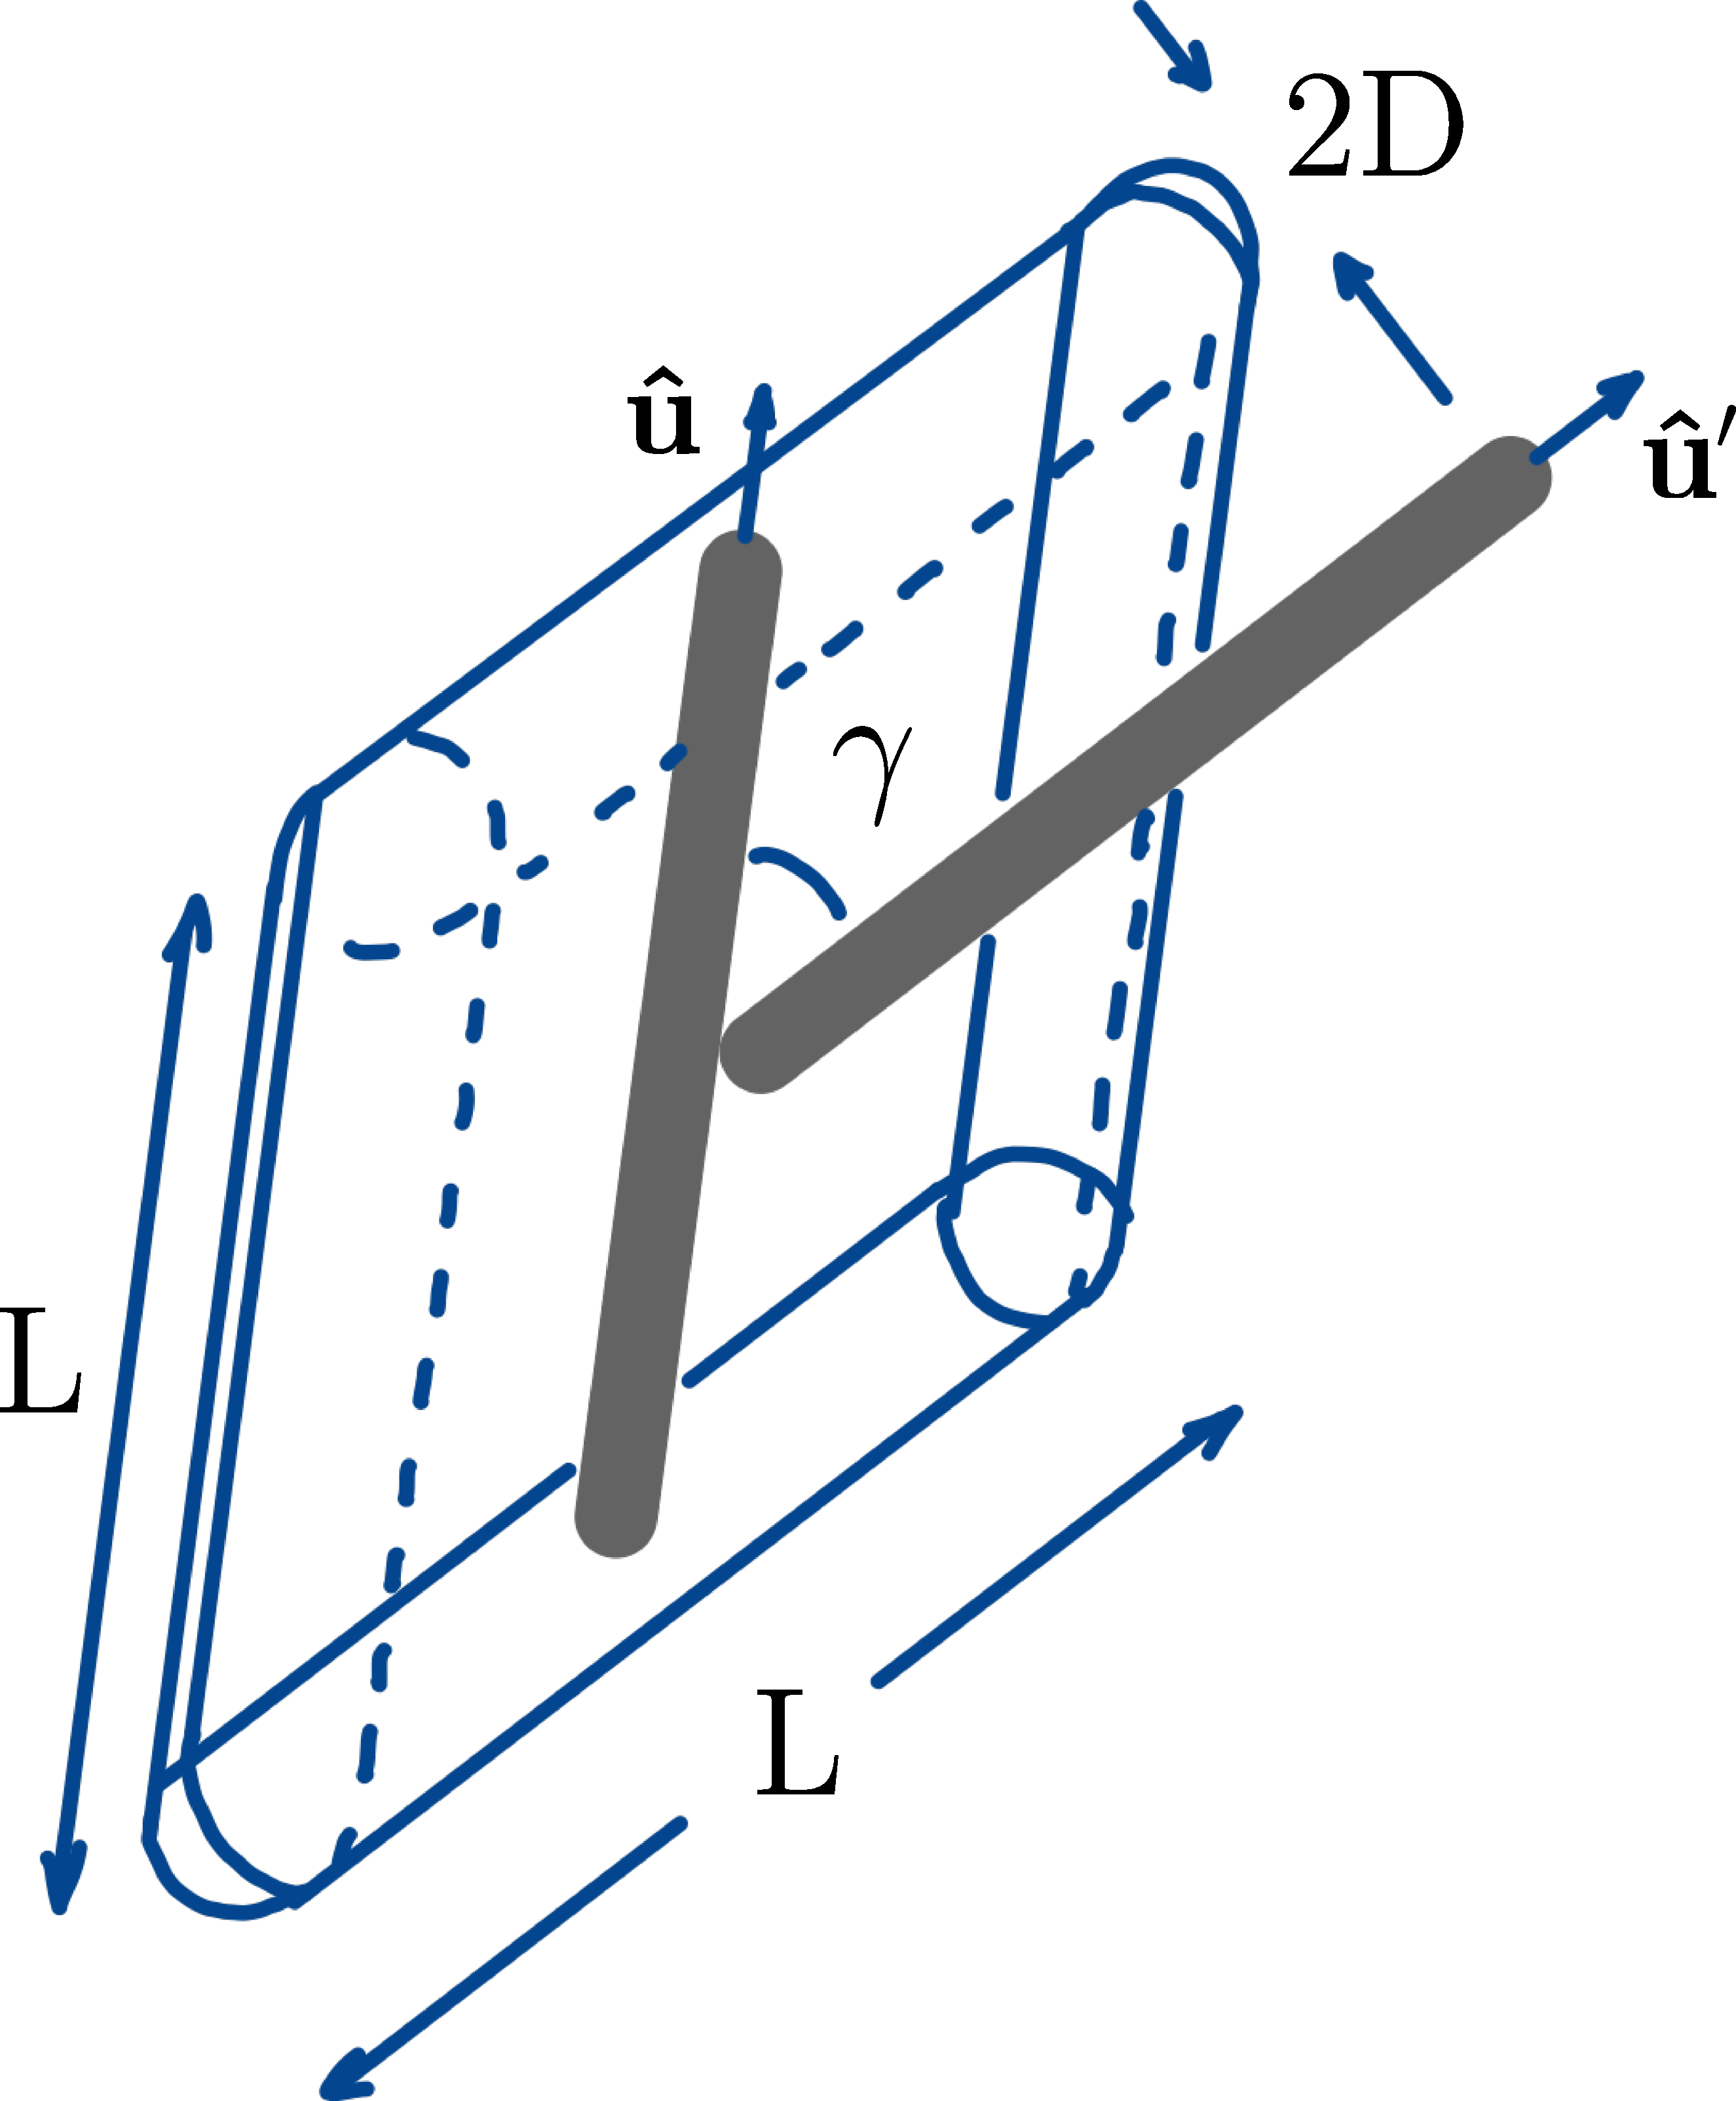
\includegraphics[width= 0.4 \columnwidth]{figures/chapter-1/exclvol}
\caption[Illustration of the excluded volume of two spherocyllinders  of length $L$ and diameter $D$ at mutual orientation $\gamma$]{ \label{introfig3} Illustration of the excluded volume of two spherocyllinders  of length $L$ and diameter $D$ at mutual orientation $\gamma$. Rod alignment leads to a strong reduction of the excluded volume represented by the lozenge-shaped figure.}
\end{SCfigure}

Since we are accounting for possible inhomogeneous angular configurations, the previous reformulation of the integral must be weighted by the ODF $f(\Omega)$.

The meaning of the excluded volume is clarified in \fig{introfig3}. Considering long hard rods we immediately infer that the excluded volume is strongly orientation-dependent; it is greatly reduced when the rods align. In consequence, taking \eq{B2_exclv} one can see that collective alignment of the rods and thus an anisotropic ODF will reduce the value of $B_2$ with respect to an isotropic state.

Lastly, we recall the free energy formulation of an imperfect gas approximated by the second virial correction:
\begin{align}
\frac{\beta F}{N} =& \beta \mu_{0}+\ln\left[\Lambda\rho\right]-1+ B_2 \rho
\end{align}
with $\mu_{0}$ a reference chemical potential of the dispersed particles depending only on the solvent conditions, and $\Lambda$ the (de Broglie) thermal volume, arising from
integrations over the translational and rotational momenta of the anisometric particles. The last term corresponds to the translational {\em entropy} in the context of Onsager's formalism, since for hard core interactions it does not depend on temperature, but only on the average over all possible configurations. Collecting the previous results from \eq{0forient} and \eq{B2_exclv} we obtain the following expression:
\begin{align}
\frac{\beta F}{N} =& \beta \mu_{0}+\ln\left[\Lambda\rho\right]-1+
\int f(\Omega)\ln \left[4\pi f(\Omega)\right]d\Omega \nonumber \\
&+\frac{\rho}{2} \iint d\Omega d\Omega^{\prime}
f(\Omega)f(\Omega^{\prime})v_{\text{excl}}(\Omega,\Omega^{\prime}). \label{0freetot}
\end{align}

This is the final recipe to model the phase behavior of an ideal mixture of hard rods, where the most probable orientational state is given by the function $f(\Omega)$ that better minimizes the Helmholtz free energy. The isotropic-nematic transition comes from a competition between the before-last and last terms, which correspond to the orientational and translational entropy respectively. For low concentrations, the orientational entropy dominates and is maximized by an isotropic distribution, whereas for high concentrations the second virial term becomes more important, which favors a nematic distribution at the expense of losing orientational entropy. The critical packing fraction at wich an isotropic-nematic ordering occurs roughly corresponds to the situation when the bare particle volume is of the same order of magnitude as its average excluded volume:

\begin{equation}
\phi_{IN} \propto \frac{\mbox{{\small volume per particle}}}{\mbox{{\small average excluded volume per particle}}}
\end{equation}

The excluded volume for a pair of spherocylinders as sketched in \fig{introfig3} reads

\begin{equation}
v_{excl}(\Omega_1,\Omega_2) = 2L^2D |\sin\gamma|+2\pi D^2 L + \frac{4}{3}\pi D^3
\end{equation}

An analogous expression was obtained by Onsager for two cylinders with different arbitrary lengths, diameters and mutual orientation \cite{onsager1949}. Simple scaling considerations for thin cylinders then prompt us to infer that, whereas the volume per particle scales as $\propto L D^2$, the excuded volume typically goes as $\propto D L^2$. In consequence,


\begin{equation}
\phi_{IN} \propto \frac{D}{L}
\end{equation}

Clearly, the more slender the rods (large $L/D$) the lower the critical packing fraction at which the I-N phase transformation can be expected. Strictly, in the Onsager limit $L/D \rightarrow \infty$ the transition occurs in the ultra-dilute regime where a pair-interaction-only approximation is entirely justified.

\subsubsection{Mixtures}

Chapter \ref{disc_polymer} will focus on mixtures of anisometric particles consisting of multiple distinct species (e.g., mixtures of discs and polymers with multiple aggregation numbers). Introducing mole fractions $x_{j}=N_{j}/N$ for each species $j$, the free energy of the mixture can be expressed as a straightforward generalization of \eq{0freetot}:

\begin{align}
\frac{\beta F}{N} &\sim \ln [\rho \bar{\Lambda}]-1 + \sum_{j} x_{j} \ln x_{j} +
\sum_{j} x_{j} \int f_{j}(\Omega)\ln \left[ 4 \pi f_{j}(\Omega) \right] d \Omega \nonumber \\
&+\frac{\rho}{2}\sum_{j}\sum_{k}x_{j}x_{k} \iint  d \Omega d\Omega^{\prime}
f_{j}(\Omega)f_{k}(\Omega^{\prime})
v_{\text{excl}}^{jk}(\Omega,\Omega^{\prime}),  \label{0freetotmulti}
\end{align}
with $\bar{\Lambda}=\prod_{j}\Lambda_{j}^{x_{j}}$. The contribution $\sum_{j} x_{j} \ln x_{j}$ represents the {\em entropy of mixing} due to the fact that we are dealing with different species. Although the free energy for mixtures can be easily established,  the implications of \eq{0freetotmulti} are quite significant. In particular, each species $j$ now has its own ODF which must be normalized according to $\int f_{j}(d\Omega)d\Omega \equiv 1$. Moreover, in the case of phase coexistence between an isotropic ($I$) and a nematic ($N$) phase, the conditions for mechanical and chemical equilibrium require equal osmotic pressure $\Pi$ and chemical potentials $\mu_{j}$ for {\em all} species involved. Thus, the coexistence equations read:

\begin{align}
\Pi^{I}&=\Pi^{N} \nonumber \\
\mu^{I}_{j}&=\mu^{N}_{j} \qquad\qquad \text{for {\em all} $j$},
\end{align}

where we must take into account that the composition ${x_{j}}$ may differ in each phase due to fractionation effects. These considerations indicate that the calculation of phase transitions in mixtures is generally a challenging task, requiring specific approximations or numerical techniques depending on the physical situation. More details on the particular approaches addressed in this research work can be found in Chapter \ref{disc_polymer} in which we discuss the case of reversibly polymerizing rods.

\subsection{Facing reality}

Going back to the experimental systems of nanorods and platelets mentioned at the beginning of this chapter it is clear that a simple hard-particle model is often too simple to arrive at a satisfactory description of a typical experimental setup. A number of extensions and modifications of Onsager's theory are then necessary. Some of them involve attempts to account for:

\begin{enumerate}
\item Multicomponent mixtures of rod, disks, or living polymers
\item Effect of external aligning fields
\item Semi-flexibility
\item Long-ranged ``soft" interactions (e.g. depletion attraction)
\item Chirality
\item Non-uniform systems (smectic membranes, interfaces, effect of solid substrates)
\end{enumerate}

In the main body of this work we will illustrate the rich phenomenology brought about by the topics listed above, most of the time as perturbations to the main entropic hard-core contribution, discussed previously in the context of Onsager's theory. We hope that these examples will convince the reader of the predictive power and versatility of Onsager's second-virial theory even when applied beyond the strict bounds of applicability as formulated in his original paper. In what follows, topics 4 and 5, albeit already introduced, are now very briefly discussed from a more quantitative perspective.

\subsubsection{Depletion}

Similar to a Yukawa potential, while the depletion interaction remains relatively tractable for simple spherical particles, the quantity becomes highly non-trivial for more complex colloidal shapes. This is due to the intrinsic orientation-dependence of the depletion zones and their overlap conditions when generalized to suspensions involving rod or disk-shaped nanoparticles, and also to the non-additive nature of the depletion potential when the size of the depletants is comparable to the width of the colloids. The depletion attraction between non-isotropic particles could be formally expressed as a mean-field correction term:


 \begin{equation}
U \sim  -\frac{1}{2} \frac{N^{2}}{V} \Pi_{dep} \left \langle \int_{
\substack{
\mbox{\tiny no core overlap,} \\
\mbox{\tiny depletion zone overlap}
}
} d {\bf r}_{ij}   v^{dep}_{ij}({\bf r}_{ij})  \right \rangle_{\mbox{\tiny orientational states of rods i and j}}
\label{degen}
\end{equation}
where $\Pi_{dep}$ is the osmotic pressure of the depletants. In arriving at this expression, the depletion agents have been considered to be mutually non-interacting and the effective attraction ptential between the nanoparticles is proportional to the overlap volume $v^{dep}_{ij}$ of the depletion zones of particles $i$ and $j$ (see \fig{introfig2}) \cite{LekkerkerkerTuinier2011}.

\subsubsection{Chirality}

The presence of surface charges (or {\em soft patches}) residing on the colloid surface in a distinctly {\em helical} distribution can impart a distinctly chiral signature on to the effective interactions between the nanoparticles. In this case, there is a supplementary soft interaction coupling to the rod orientation vector $\bhu$ of each rod $i$ and $j$ (see \fig{introfig1} (e) and (f)) and their centre-of-mass distance vector $\bf r$ through the following pseudo-scalar expression \cite{goossens1971}:
\beq
u_{ij} \sim  \varepsilon_{c} g( r)({\bf \hat{u}}_{i} \cdot {\bf \hat{u}}_{j}) ( {\bf \hat{u}}_{i} \times {\bf \hat{u}}_{j} \cdot {\bf r} )
\label{chirality}
\eeq

In Chapter \ref{twistedrods}, we will analyze in detail the implications of this interaction for the chiral features of colloidal mesoscopic compounds, whose microscopic details can be encapsulated into the effective chiral amplitude $\varepsilon_c$ and decay function $g(r)$, which express the typical range over which chiral forces are transmitted. The effective potential is distinctly chiral and lacks inversion symmetry, meaning that it changes under a transformation ${\bf r}_{ij} \rightarrow -{\bf r}_{ij} $, while preserving basic head-tail symmetry $u_{ij}({\bf \hat{u}}_{i/j}) = u_{ij}(-{\bf \hat{u}}_{i/j}) $.

\section[HPMC simulations of colloidal nematics]{Hard-particle Monte Carlo simulations of colloidal nematics: some technical details}

In the last half century, the use of molecular simulations has become increasingly widespread across a multitude of scientific disciplines, representing an essential tool in the realm of colloidal and soft matter science. The initial success of these simulations can be traced back to their ability to predict the transition between the liquid and solid phases in a system of hard spheres \cite{ALDER57,WOOD57}. Since then, molecular simulations have become a pillar in soft matter research, allowing for the exploration of complex systems at the molecular level with remarkable accuracy and versatility.

Molecular simulations are classified into two principal categories: Molecular Dynamics (MD) and Monte Carlo (MC) simulations. The fundamental aim of both techniques is to acquire macroscopic observables from microscopic properties of the system. While MD simulations focus on time averages, MC simulations rely on ensemble averages. In the thermodynamic limit, these two types of averages become equivalent, according to the ergodic hypothesis, which postulates that a system traverses all possible states in its phase space over a long enough time scale \cite{dfrenkel96:mc}. As a result, the use of molecular simulations has led to significant advances in a variety of fields, ranging from materials science to biophysics and beyond, making them an indispensable tool for contemporary scientific research.

One of the advantages of MC over MD is that it permits to study systems characterized by non-analytical interaction potentials e. g. the hard core interaction invoked in this work. Using Monte Carlo simulations to explore the configurational space of a system at certain conditions, an observable $A$ can be calculated as an average over a big number of accessible configurations. In the canonical ensemble (systems at constant $\{N,V,T\}$) this can be integrated using the Boltzmann probability of finding a particle configuration of energy U, $\exp( -U/k_{B}T)$:

\beq
\langle  A \rangle = \frac{\int d \bfr^NA(\bfr^N)\exp(-\beta U)}{\int d \bfr^N\exp(-\beta U)}
\label{observable}
\eeq

A possible way to evaluate \eq{observable} is through the Metropolis Monte Carlo algorithm \cite{Metropolis1953}, which becomes much simpler for hard core systems due to the fact that, in this case, the Boltzmann factor can only be worth 0 or 1. The basic form of a MC cycle then becomes:


\begin{algorithm}[h]
    \SetAlgoLined

    Start from an initial configuration of $N$ particles\;
    \For{$k = 0,\dots,N-1$}{
        Choose a random particle $i$\;
        Give the particle a random transformation (translation or rotation)\;
        Check for overlaps\;
        \eIf{new configuration generates an overlap}{
            Reject: roll back to old configuration\;
        }{
            Accept: update the configuration\;
        }
    }
    \caption{Metropolis Monte Carlo algorithm for hard--core potentials in the canonical ensemble.}
    \label{algo:MHPMC}
\end{algorithm}


In this section we aim to give an overview of the technical peculiarities of Hard Particle Monte Carlo (HPMC) simulations of anisotropic particles, in particular mixtures of elongated rods and depletants, that are used in the computational model studied in Chapter \ref{twistedrods}.

\subsection{Overlap conditions for hard spherocyllinders}

As shown in Algorithm~\ref{algo:MHPMC}, in HPMC a move is accepted if there is no overlap between two particles. Hence an efficient overlap test is key in this technique. In the case of spherical objects the overlap test is very simple: it is enough to compute the distance between the center of the two spheres $r_{ij}$ and verify that it is less than the sum of their radii: $r_{ij} \leqslant R_i + R_j$ or, in a computationally cheaper form, $r_{ij}^2 \leqslant (R_i + R_j)^2$. It is possible to model elongated hard rods that use this simple overlap condition by building particles composed of spherical objects attached in a linear chain. In this case, the overlap test simply consists on evaluating pairs of spherical objects associated to distinct rods. However, the computational expense of this strategy is enormous as it involves the order of $N_b^2$ operations at each MC move where $N_b$ is the number of spherical beads in one rod.

This problem is overcome if each colloidal rod is considered to be a spherocylinder, for which a more efficient overlap test is proposed by Allen {\em et al.} \cite{allenevans93}. The key steps are outlined below.

A spherocylinder $i$ is defined by its cylindrical surface length $L$, the diameter $D$ of its cylindrical surface and its two hemispheres, the coordinates $\bfr_i$ of its center of mass and the unit vector $\bhu_i$ indicating its orientation. We want to determine the minimum distance between the cores of two spherocylinders $i$ and $j$ with equal lengths and diameters. We can describe any point of the line segment core of $i$ and $j$ parametrically as

\begin{align}
\bfr_i(\lambda) &= \bfr_i + \lambda \bhu_i \nonumber \\
\bfr_j(\mu) &= \bfr_j + \mu \bhu_j
\end{align}

In order to calculate the minimum distance between two arbitrarily oriented lines we can take advantage of the fact that the shortest distance vector,
\beq
\bfr_{ij}^{min}(\lambda_0,\mu_0)=\bfr_{j}(\mu_0)-\bfr_{i}(\lambda_0),
\eeq
must be perpendicular to both $\bhu_i$ and $\bhu_j$. Assuming $\bfr_{ij}^{min}(\lambda_0,\mu_0) \cdot \bhu_i = 0$ and $\bfr_{ij}^{min}(\lambda_0,\mu_0) \cdot \bhu_j = 0$ we obtain a system of equations that we can solve to get the minimizing values $\lambda_0$ and $\mu_0$:
\beq
\begin{pmatrix}
\lambda_0 \\
\mu_0
\end{pmatrix}
= \frac{1}{1-(\bhu_i \cdot \bhu_j)^2}
\begin{pmatrix}
-\bhu_i \cdot \bfr_{ij} + (\bhu_i \cdot \bhu_j)(\bhu_j \cdot \bfr_{ij}) \\
+\bhu_j \cdot \bfr_{ij} + (\bhu_i \cdot \bhu_j)(\bhu_i \cdot \bfr_{ij})
\end{pmatrix}
\label{overlapeq}
\eeq
where $\bfr_{ij} = \bfr_{j} - \bfr_{i}$ is the distance between centers of mass. Since for line segments $-\frac{L}{2} \leqslant (\lambda,\mu) \leqslant \frac{L}{2}$ we have to truncate the result of \eq{overlapeq} if it exceeds this limit. In order to avoid more arithmetical operations than necessary, at this point it is better to compute the square minimal distance
\begin{align}
(\bfr_{ij}^{min})^2(\lambda_0,\mu_0) = \bfr_{ij}^2& + \lambda_0^2 + \mu_0^2 - 2\lambda_0\bhu_i \cdot \bfr_{ij} \nonumber \\
    & + 2\mu_0\bhu_j \cdot \bfr_{ij}  - 2\lambda_0\mu_0\bhu_i \cdot \bhu_j
\end{align}
from quantities already calculated. All the above scheme works unless shperocylinders are completely parallel to each other, in which case \eq{overlapeq} is not well defined. We can add a condition to account for this particular case, where the minimal distance would be simply calculated as the distance between two parallel lines.

There is an overlap between the two spherocylinders if $(\bfr_{ij}^{min})^2 \leqslant D^2$. A generalization of this idea can be done for mixtures of two different species of spherocylinders of lengths $L_{1,2}$ and diameters $D_{1,2}$ by simply rewriting
\begin{align}
-\frac{L_i}{2}& \leqslant \lambda \leqslant \frac{L_i}{2} \nonumber \\
-\frac{L_j}{2}& \leqslant \mu \leqslant \frac{L_j}{2} \nonumber \\
    (\bfr_{ij}^{min})^2& \leqslant \left( \frac{D_i+D_j}{2}\right)^2
\end{align}
where $i,j=$ 1 or 2 if the spherocylinders belong to the first or second species respectively. For mixtures of spherocylinders and spheres, the expressions can also be valid by taking $L=0$ for spheres.

\subsection{Semi-grand canonical ensemble}

Several theories have been developed that enable calculations of phase transitions in systems with depletion interactions. The free volume theory (FVT) by Lekkerkerker {\em et al.} \cite{sphere+polymer} for the phase behavior of dispersions of colloids and non-adsorbing polymer was the first one to account for depletant partitioning over the coexisting phases. This theory is based on the osmotic equilibrium between two systems: a hypothetical depletant reservoir and a mixed colloid $+$ depletant system. Because of its affordability in terms of complexity and yet a phenomenologically accurate description of the problem, this theory serves as a standard reference today, both for theoretical and computational models.

The starting point is the {\em semi--grand} potential density of a system of colloids and polymer in equilibrium with a reservoir containing only the polymer. This semi--grand potential is separated into a hard colloid contribution and a polymer contribution. The colloid part may be described by known expressions for the colloidal fluid and crystalline phases in the canonical ensemble (fixed volume, temperature and number of colloidal particles $\{N,V,T\}$). The polymer contribution is found from a build-up principle: starting from a system without polymer, chains are added to the system until the final concentration is reached, and the polymer contribution is calculated by integrating along this path. This is the reason why the polymer part is treated in a more natural way by using the grand canonical formalism (fixed volume, temperature and polymer chemical potential $\{\mu_p,V,T\}$). The key assumption of this theory is that thermodynamic quantities can be calculated for both colloids and depletants from their independent ensembles, correlated only by means of an ensemble--averaged free volume for the depletants in the mixed system $\langle V_{free} \rangle$. As a result, we can define

\beq
\Omega(N,V,T,\mu_p) = F_0(N,V,T) - \Pi^R\langle V_{free} \rangle
\eeq
where $F_0$ is the free energy of the colloidal particle system without added depletant, $\mu_p$ represents the chemical potential of the polymer depletant and $\langle V_{free} \rangle$ is the available volume for the depletants, i.e. the total volume in the mixed system outside the depletion layers, and it is approximated by the free volume in the pure hard colloid dispersion $\langle V_{free} \rangle_0$. This approximation is valid in the limit of low depletant activity, and starts losing accuracy when increasing it. $\Pi^R$ is the osmotic pressure in the reservoir, and it can be easily calculated by considering the depletants as penetrable hard spheres, which allows for a real gas formulation and thus

\beq
\Pi^R=n_pk_BT
\eeq
where $n_p$ is the number density of the depletants in the reservoir. We can also write the chemical potential:

\beq
\mu_p = \textrm{const} + k_BT\ln n_p
\eeq

In order to equate the depletant chemical potentials in both systems, we infer that the average number of depletants in the mixed system $N_p$ must fulfill
\beq
N_p= n_p\langle V_{free} \rangle
\eeq

In what matters to our simulations presented in Chapter \ref{twistedrods}, the total number of particles in a semi-grand MC scheme is no longer constant, but rather fluctuating towards an optimal value given by $N + N_p$. This allows us to stabilize mesoscopic colloidal compounds while maintaining a constant depletion pressure. Algorithm \ref{algo:MHPMC} is then rewritten as:

\begin{algorithm}[h]
    \SetAlgoLined

    Start from an initial configuration of $N$ colloids and $N_p$ depletants\;
    \For{$k = 0,\dots,N + N_p -1$}{
    Choose a random particle type\;
        \If{type is colloid}{
            Choose a random particle $i$\;
            Give the particle a random transformation (translation or rotation)\;
            Check for overlaps\;
            \eIf{new configuration generates an overlap}{
                Reject: roll back to old configuration\;
            }{
                Accept: update configuration\;
            }
        }
        \If{type is depletant}{
            Choose a random transformation (insertion or deletion)\;
            \If{insertion}{
                Generate random coordinates\;
                Check for overlaps\;
            \eIf{new configuration generates an overlap}{
                Reject: roll back to old configuration\;
            }{
                Insert with probability
                \beq
                    \sim \frac{V}{\Lambda(N_p+1)}e^{\beta\mu_p}\; \nonumber
                \eeq
            }

            }
            \If{deletion}{
                Choose a random particle $i$\;
                Delete with probability
            \beq
                \sim \frac{\Lambda N_p}{V}e^{-\beta\mu_p}\; \nonumber
            \eeq
            }
            Update $N_p$ if necessary\;
        }
    }
    \caption{Semi--grand canonical Monte Carlo scheme for mixtures of $N$ colloids $+$ depletants at constant chemical potential $\mu_p$. }
    \label{algo:semiHPMC}
\end{algorithm}

Similar schemes have been performed by Bolhuis and Frenkel \cite{Bolhuis1994} and Vink and Horbach \cite{Vink2004}. Both of these works employ cluster moves as a strategy to increase the acceptance ratio of these MC simulations, which is otherwise significantly low since trial depletant insertion moves have a high probability of overlapping with the volume occupied by the colloids.

\subsection{Implicit depletants algorithm}
\label{sec:implicit}

In the previous approach, simulation performance can become compromised due to the need to explicitly track all the depletant particles. This is particularly evident in our simulations where a large region of the system volume needs to be kept empty around the mesoscopic colloidal droplets to prevent artifacts induced by system boundaries. As a result, a significant portion of the total volume is completely filled with depletants, which need to be stored and updated during the simulation and yet are not relevant for subsequent statistical analysis.

Some approaches that aim to overcome this issue (\cite{bolhuis_jcp1997,PhysRevE.73.041404,Henzie2011} to name a few) are based on a effective depletion potential approach, integrated over all the depletant degrees of freedom. However, achieving sufficient accuracy in the pairwise effective potential also comes at the expense of computation time, whereas an overly simplified interaction may hinder the study of arbitrary shapes and size ratios.


\begin{algorithm}[h]
    \SetAlgoLined

    Start from an initial configuration $M$ of $N$ colloidal particles\;
    \For{$k = 0,\dots,N-1$}{
        Choose a random particle $i$\;
        Give the particle a random transformation (translation or rotation). Let $M^\prime$ be the new system configuration\;
        Check for overlaps\;
        \eIf{overlap in $M^\prime$}{
            Reject: roll back to $M$\;
        }{
            According to the Poisson probability distribution
            \beq
            \sim \text{Poisson}(\frac{V_{free}}{\Lambda}e^{-\beta\mu_p}) \nonumber
            \eeq
            of mean and variance $\frac{V_{free}}{\Lambda}e^{-\beta\mu_p}$, choose a number of depletants $N_p$ that will be generated\;
            Generate $N_p$ random depletant positions in $V_{free}$ the free volume of $M$\;
            Check for overlaps between $M^\prime$ and the generated depletant positions\;
            \eIf{overlap}{
                Reject: roll back to $M$\;
            }{
                Accept: update to $M^\prime$\;
            }
        }
    }
    \caption{General implicit depletant algorithm proposed by \cite{glaser2015parallel}.}
    \label{algo:implicit}
\end{algorithm}

Glaser {\em et al.} \cite{glaser2015parallel} proposed a scheme to handle many-body depletion interactions implicitly, avoiding the need to simulate a large number of particles, while maintaining a particle-based approach instead of a more complex effective pairwise potential. The fundamental idea behind this scheme is that depletants can be treated as an ideal gas, assumed to be statistically independent, and therefore, they can be randomly inserted into the excluded volume surrounding a single translated or rotated colloid for each MC step. These depletants are then discarded and re-generated at the following step. The algorithm is particularly efficient for dilute systems of colloids and a large expected number of depletants. It obeys detailed balance and can accept further multi--core parallel implementations.

In a nutshell, Algorithm \ref{algo:implicit} conveys the basic idea of this scheme in its most general form. However, this version is computationally impractical since it requires integration of the free volume $V_{free}$ in the entire simulation box for every single colloid move. In the original article \cite{glaser2015parallel} several alternative volume choices are considered, and proved to obey detailed balance. It is possible to choose a smaller region $V_0 \subset V$ of the entire volume, containing only the region where modifications are being applied. For simplicity, this volume can also contain regions in principle unaccessible to depletants, i. e. $V_0 \setminus (V_0 \cap V_{free}) \neq \emptyset$; it suffices to ignore the colloid-polymer overlaps occuring in these regions.

For anisotropic colloids with aspect ratios $\sim 1$, \cite{glaser2015parallel} proposes to choose $V_0$ as the circumsphere of diameter $D_{colloid} + D_{depletant}$ around the colloid in the new configuration $M^\prime$, ignoring depletants that overlap with the colloid in the old configuration $M$. In our case, due to the large aspect ratios that we will be dealing with, we shall rather define $V_0$ more conveniently as a cylinder at the center of mass of the moved colloid $i^\prime$, with diameter $D + a$, length $L + D + a$ (with $a$ being the depletant diameter) and orientation $\bhu_i^\prime$. See \fig{implicit} for a depiction of our approach.

\begin{figure}
\begin{center}
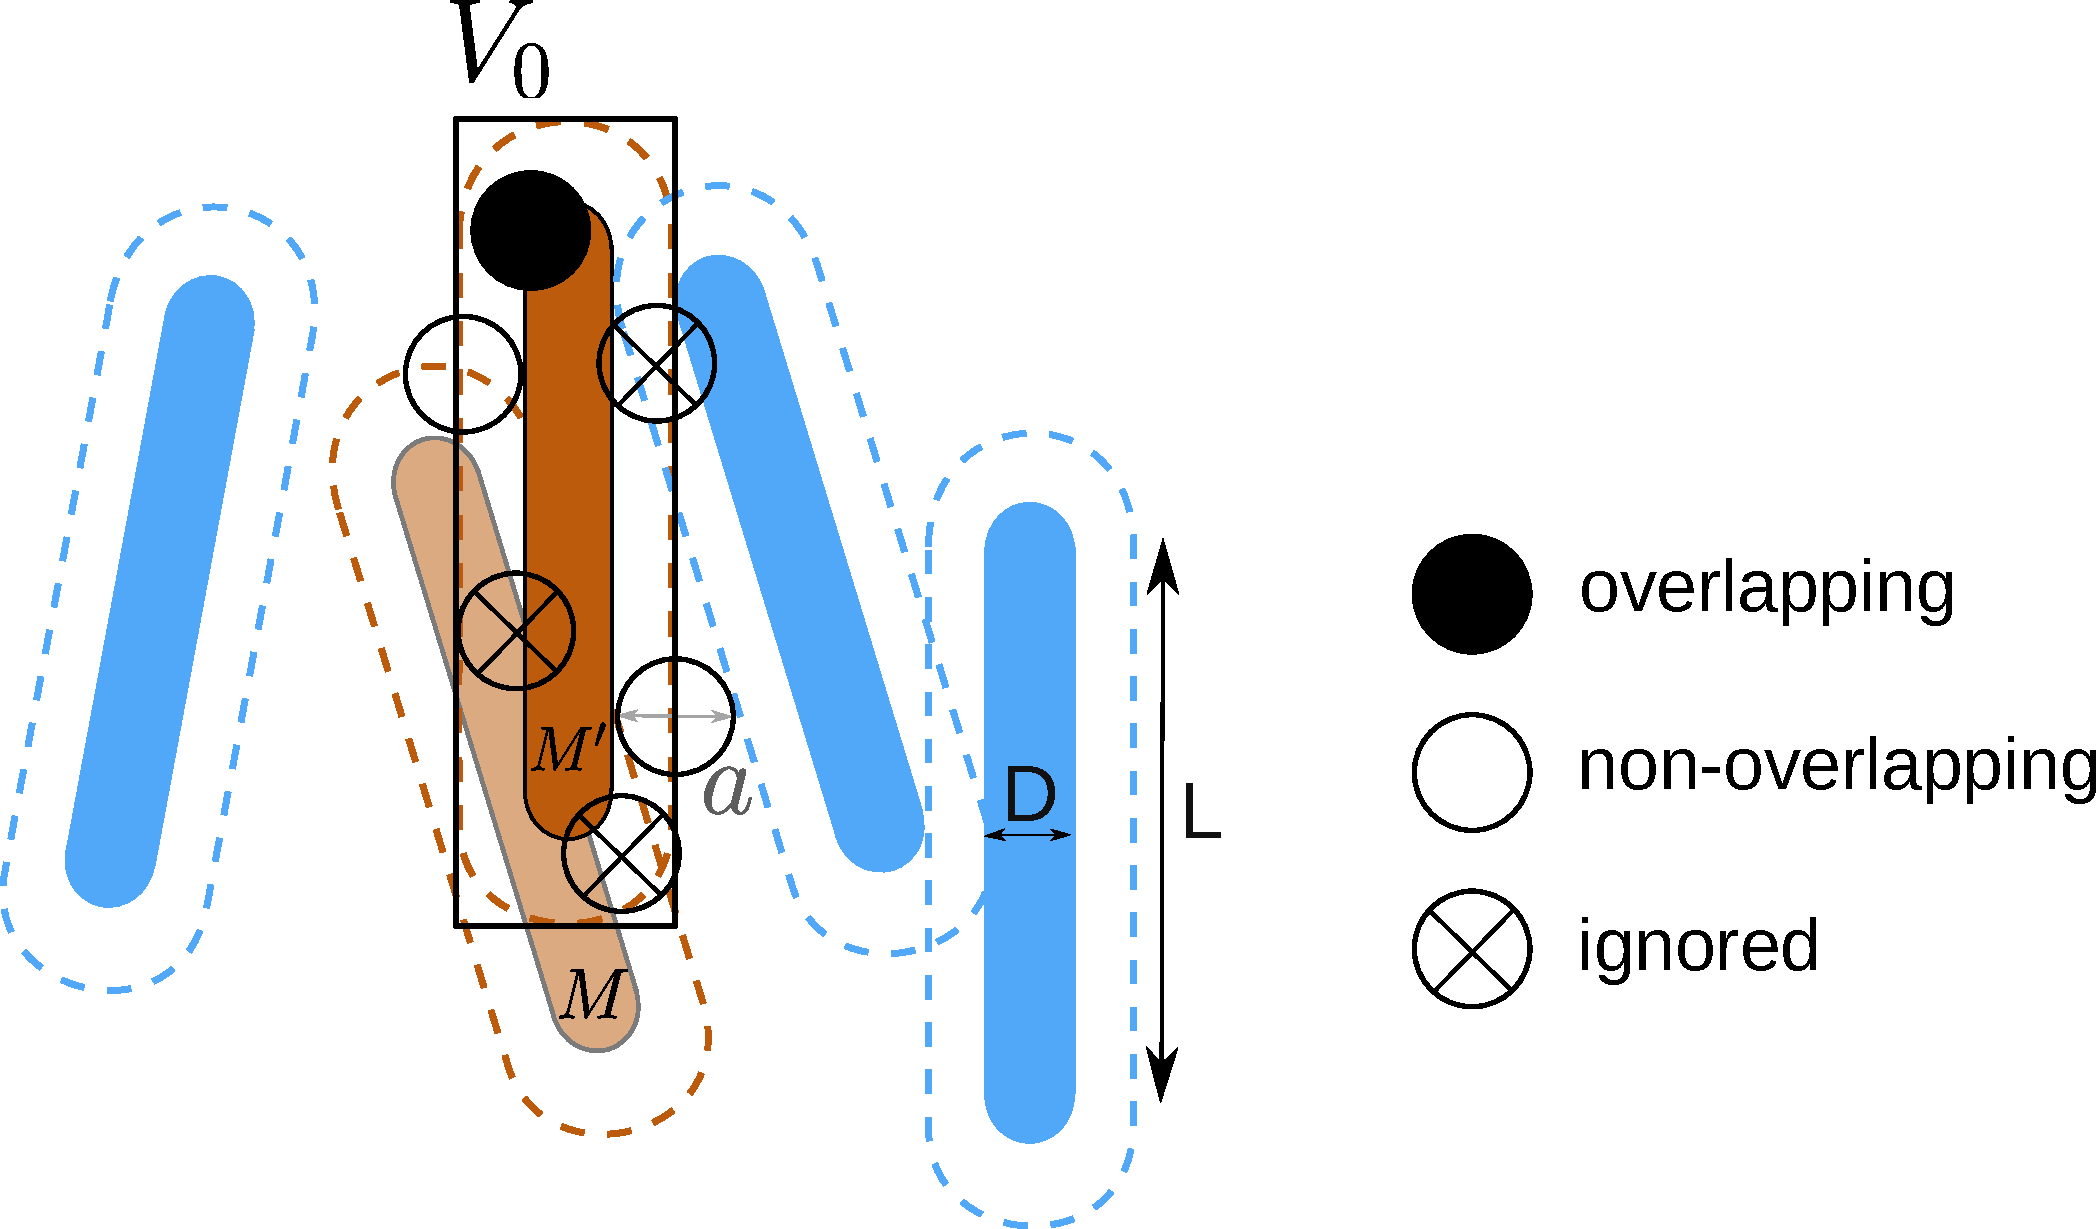
\includegraphics[width= .8\columnwidth]{figures/chapter-1/implicit_depletants}
\caption[Depletant positions (spheres) considered for rejection of a colloid move (orange spherocyllinders)]{ \label{implicit} Depletant positions (spheres) considered for rejection of a colloid move (orange spherocyllinders). When updating the configuration, depletants are randomly inserted into the cylinder (black rectangle) containing the excluded volume between the colloid and the depletants. Overlapping depletants (black spheres) lead to rejection of the trial move. Depletants that overlap with the old position $M$ or with surrounding colloids (blue) are not considered.}
\end{center}
\end{figure}

\clearpage